
This study applies machine learning techniques to classify bacterial exotoxins based on their functional types and biological targets.
The methodology follows a structured pipeline that involves data collection, preprocessing, feature extraction, and model training.

First, primary sequences was collected and analyzed using descriptive statistics to understand key sequence characteristics. Next, the dataset was preprocessed using redundancy reduction techniques to generate a non-redundant set of sequences.
Next, protein language models were used to generate numerical embeddings that capture meaningful sequence representations.

Subsequently, dimensionality reduction using Principal Component Analysis is applied to the embeddings. The processed embeddings are then used to train machine learning models, including conventional classifiers and hierarchical predictors. The machine learning models are evaluated using performance metrics for binary and multiclass classification tasks. 

Figure~\ref{fig:methods_workflow} visualizes the key steps in building a machine learning classification pipeline for differentiating exotoxin types and targets.

\begin{figure}[htbp]
	\centering
	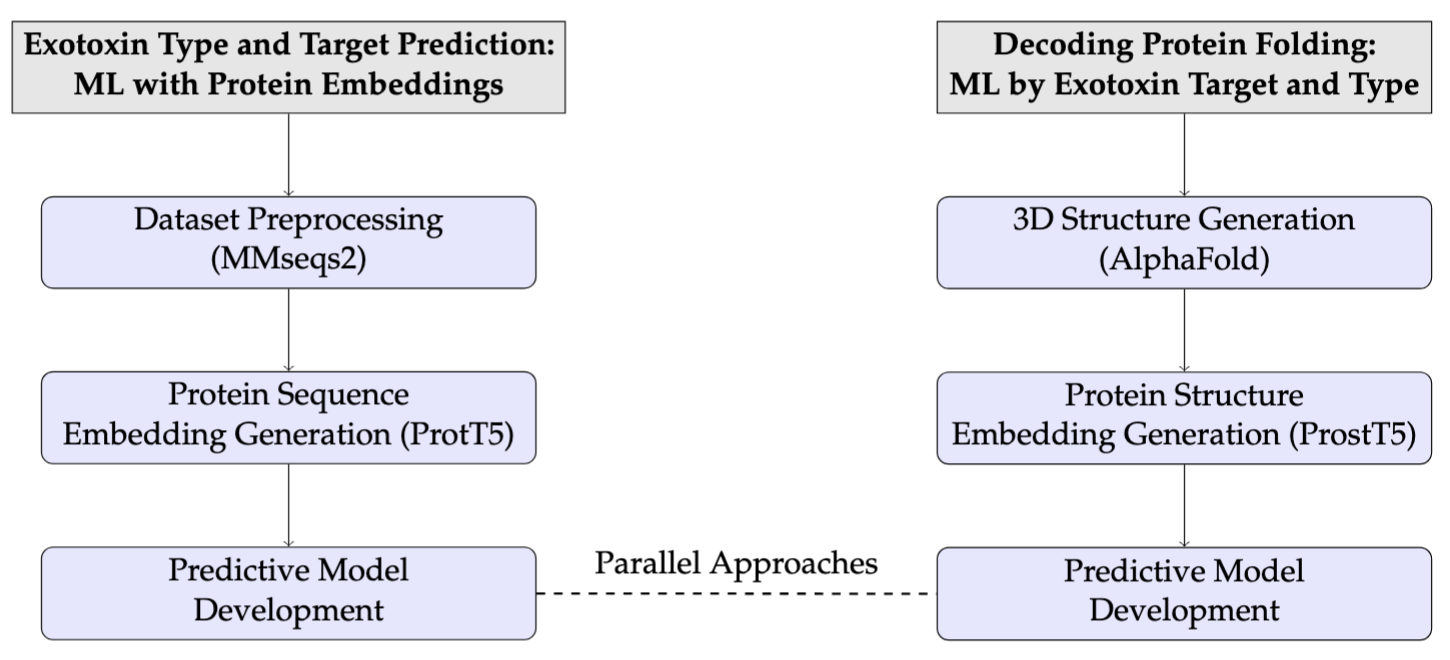
\includegraphics[width=1.1\textwidth]{images/workflow_methods.png}
	\caption{Overview of the key steps in the methodology: Exotoxin type and target predictions based on protein (left) and protein folding-based classification (right).}
	\label{fig:methods_workflow}
\end{figure}

\section{Data Collection and Curation}

Bacterial toxins protein sequences were collected from public sequence databases, such as UniProt and NCBI, as decribed previously by Krueger et al \cite{kruger2024toxin}. The dataset was curated and labeled by selecting proteins from bacterial pathogens based on their host specificity by PD. Dr. Luisa F. Jimenez-Soto.
Proteins from bacterial pathogens affecting insects, plants, and other bacteria were categorized as non-vertebrate targets, whereas proteins from bacterial pathogens affecting vertebrates—including fish, amphibians, birds, reptiles, and mammals—were classified as vertebrate targets. 

Similarly, bacterial exotoxins were categorized based on their mode of action on how they exert their effect on the host. Bacterial exotoxins were classified into different functional types, including membrane-transducing toxins, pore-forming toxins, intracellular toxins, and toxins that degrade the extracellular matrix.

\subsection{Dataset Structure and Preprocessing}
The curated dataset was structured in a CSV file, which contains bacterial species, their exotoxin types, and their specific targets. This labeled data was used to annotate the input files to build a predictive model for classifying bacterial exotoxins.

The FASTA file stores each exotoxin ID alongside its corresponding protein sequence. To integrate these datasets, the CSV and FASTA files were merged using their IDs. The resulting fully labeled dataset includes bacterial exotoxin sequences along with their respective types and targets. This data preprocessing step is implemented in the \texttt{data-preprocessing.py} script using Python 3.13.1.

Then, a Python script was employed to eliminate sequences annotated as 'partial' or 'fragment' in their FASTA headers, thereby reducing incomplete sequences.

\subsection{Dataset Composition}
The final dataset contains 2,473 sequences. Type III toxins have 2,148 entries, including both Type III and Type III Control. Type II toxins have 169 entries, including Type II and Type II PFT bacteria. Type I toxins have 42 entries, while Type IV toxins have 28 entries. An additional 104 entries are categorized as Unknown, as they do not belong to any of the four existing classes.

The target category consist of vertebrate-targeting exotoxins and non-vertebrate-targeting bacterial exotoxins, with 1,863 and 629 data points, respectively.

\section{Descriptive Statistical Analysis of Sequences}
\label{section:descriptive_statistical_analysis}

Understanding the statistical properties of protein sequences is essential for analyzing their biological characteristics and identifying potential biases in the dataset. Descriptive statistical analysis provides insights into fundamental sequence properties, such as length distributions and hydrophobicity.

This analysis was conducted using custom Python scripts, incorporating key libraries such as Biopython 1.85 for sequence handling, NumPy 2.2.2 for numerical computations, and Matplotlib 3.10.0 for visualization. 

\subsection{Mean Sequence Length}
\label{subsection:mean_sequence_length}

Understanding length variability is crucial, as it may influence the training of machine learning models. The mean sequence length $\mu$ was calculated by using the following formula:

\begin{equation}
	\mu = \frac{1}{N} \sum_{i=1}^{N} L_i
	\label{eq:mean_sequence_length}
\end{equation}

where:
\begin{itemize}
	\item $\mu$ is the mean sequence length,
	\item $N$ is the total number of sequences in the dataset,
	\item $L_i$ represents the length of the $i^{th}$ sequence.
\end{itemize}

\subsection{Hydrophobicity Analysis}
\label{subsection:hydrophobicity}

Hydrophobicity affects protein structural stability, folding, and interactions with cellular components \cite{Baldwin2007}. The average hydrophobicity $H$ of each sequence was computed using the Kyte-Doolittle scale \cite{Kyte1982}:

\begin{equation}
	H = \frac{1}{L} \sum_{i=1}^{L} H_i
	\label{eq:hydrophobicity}
\end{equation}

where:
\begin{itemize}
	\item $H$ represents the average hydrophobicity of the sequence,
	\item $L$ is the sequence length,
	\item $H_i$ is the Kyte-Doolittle hydrophobicity score of the $i^{th}$ amino acid.
\end{itemize}

These characteristics can help identify statistical outliers and reveal potential biases in the dataset.

\section{Redundancy Reduction}
\label{section:redundancy_reduction}

Machine learning models trained on redundant sequences may become biased toward overrepresented patterns, reducing their generalizability. To mitigate this, redundancy reduction was applied to the dataset using MMseqs2\cite{steinegger2017mmseqs2}.

The redundancy reduction process involved the following steps:

\begin{enumerate}
	\item The protein sequences, originally stored in FASTA format, were converted into an MMseqs2 database format to facilitate clustering.
	
	\item An initial clustering step was performed using a sequence identity threshold of 100\% . This step ensured that exact duplicate sequences were removed, preventing redundant entries in the dataset. The following command was executed:

	\texttt{mmseqs easy-cluster file.fasta dataset tmp --min-seq-id 1.0 --cov-mode 0 -c 1.0}

	\item After removing exact duplicates, a second clustering step was applied using a sequence identity threshold of 30\%. This step grouped similar sequences into clusters. The following command was used:
	
	\texttt {mmseqs easy-cluster file.fasta dataset tmp --min-seq-id 0.3 --cov-mode 0 -c 1.0}

\end{enumerate}

\section{Prediction of 3D Protein Folds}
\label{section:protein_folds}

After applying redundancy reduction to the protein sequences, their three-dimensional (3D) structures were predicted using AlphaFold2. The structural confidence of these predicted protein folds is quantified using the per-residue \textit{predicted Local Distance Difference Test} (\textit{pLDDT}) score. The pLDDT scores were used for exploratory purposes and no threshold was set based on pLDDT scores.

\subsection{Extraction of Confidence Scores from AlphaFold2 Predictions}

To evaluate the quality of the generated protein folds, a computational pipeline was developed to extract per-residue \textit{pLDDT} scores from the predicted structures. This analysis was implemented using Python and the \texttt{Biopython} library that allows the parsing of Protein Data Bank (PDB) files. The processing pipeline consists of the following steps:

\begin{enumerate}
	\item The program iterates through all PDB files generated by AlphaFold2, stored in the directory where each file corresponds to a single predicted protein structure.
	\item The script employs the PDBParser module from \texttt{Biopython} to parse the structural information of each protein model. The pLDDT score is stored within the B-factor field of each atom in the PDB file. Since all atoms within a residue share the same pLDDT value, only one atom per residue is used to extract this confidence score.
\end{enumerate}

\section{Preparation of Training and Test Datasets}
\label{section:training_test_set}

Two different methods were applied to create the training and test datasets, in order to utilize redundancy reduction to minimize sequence similarity biases and mitigating effects of data imbalance.

\subsection{Method 1: Similarity-Based Data Splitting}

After applying redundancy reduction with a sequence identity threshold of 30\%, sequences that exhibited more than 30\% similarity to any other sequence were excluded from the training set. This approach ensures that the training dataset consists of unique sequences.
Sequences with more than 30\% sequence similarity were designated as the test set. Conversely, sequences with less than 30\% similarity were assigned to the training set, forming a non-redundant subset for model learning.

\subsection{Method 2: Random Splitting After Redundancy Reduction}

In the second approach, sequences that had more than 30\% similarity were first removed from the training set, similar to Method 1. However, instead of directly assigning similar sequences to the test set, the remaining non-redundant sequences were randomly split into training and test sets.

A stratified random split was performed using the train\_test\_split function from Scikit-Learn 1.6.1, with a test size of 20\% and a random state of 42 to ensure reproducibility:

\texttt{X\_train, X\_test, y\_train, y\_test = train\_test\_split(X, y,
	test\_size=0.2, random\_state=42)}

\section{Embedding Generation}
\label{section:embedding_generation}

In this study, protein embeddings were generated from both protein sequences and protein folds, utilizing protein language models: ProtT5 and ProstT5.

For protein sequence based protein embedding generation, I employed the ProtT5 language model to generate embeddings for each protein sequence which encodes protein sequence features\cite{elnaggar2021prottrans}. A Google Colab script called embed\_ProtT5.ipynb was used during embedding generation.  

To incorporate structural information, embeddings were also generated using the ProstT5 language model from protein folds, which is trained to encode 3D structural features of proteins \cite{heinzinger2023prostt5}. A Google Colab script called ProstT5.ipynb was used during embedding generation.

\section{Dimensionality Reduction}
\label{section:dimensionality_reduction}

To reduce the complexity of embedding vectors while preserving essential information, Principal Component Analysis (PCA) was employed. PCA transforms the high-dimensional embeddings into a lower-dimensional space by keeping maximum variance. \cite{greenacre2022pca}

\section{Machine Learning Model Training and Evaluation}
\label{section:ml_training_evaluation}

To ensure robust model validation, 5-fold cross-validation was applied, and Matthews Correlation Coefficient (MCC) was used as a primary metric for model evaluation.

\subsection{Model Selection}
\label{subsection:model_selection}

Several machine learning algorithms were selected for the classification tasks. The models used in this study include:

\begin{itemize}
	\item Random Forest  \cite{Breiman2001}
	\item Logistic Regression  \cite{Cox1958}
	\item Support Vector Machine (SVM)  \cite{Cortes1995}
	\item K-Nearest Neighbors (KNN)  \cite{Guo2003}
\end{itemize}

\subsection{Additional Approach: Hierarchical Predictor}
\label{subsection:hierarchical_model}

To address class imbalances and improve classification accuracy, a hierarchical predictor was implemented. This approach first uses a classifier to group exotoxins into broader type families based on their prevalence. A second-stage classifier is then applied within each group to classify specific exotoxin types with similar datapoints. The architecture of this predictor is depicted in Figure~\ref{fig:hier_logic} below.

\begin{figure}[htbp]
	\centering
	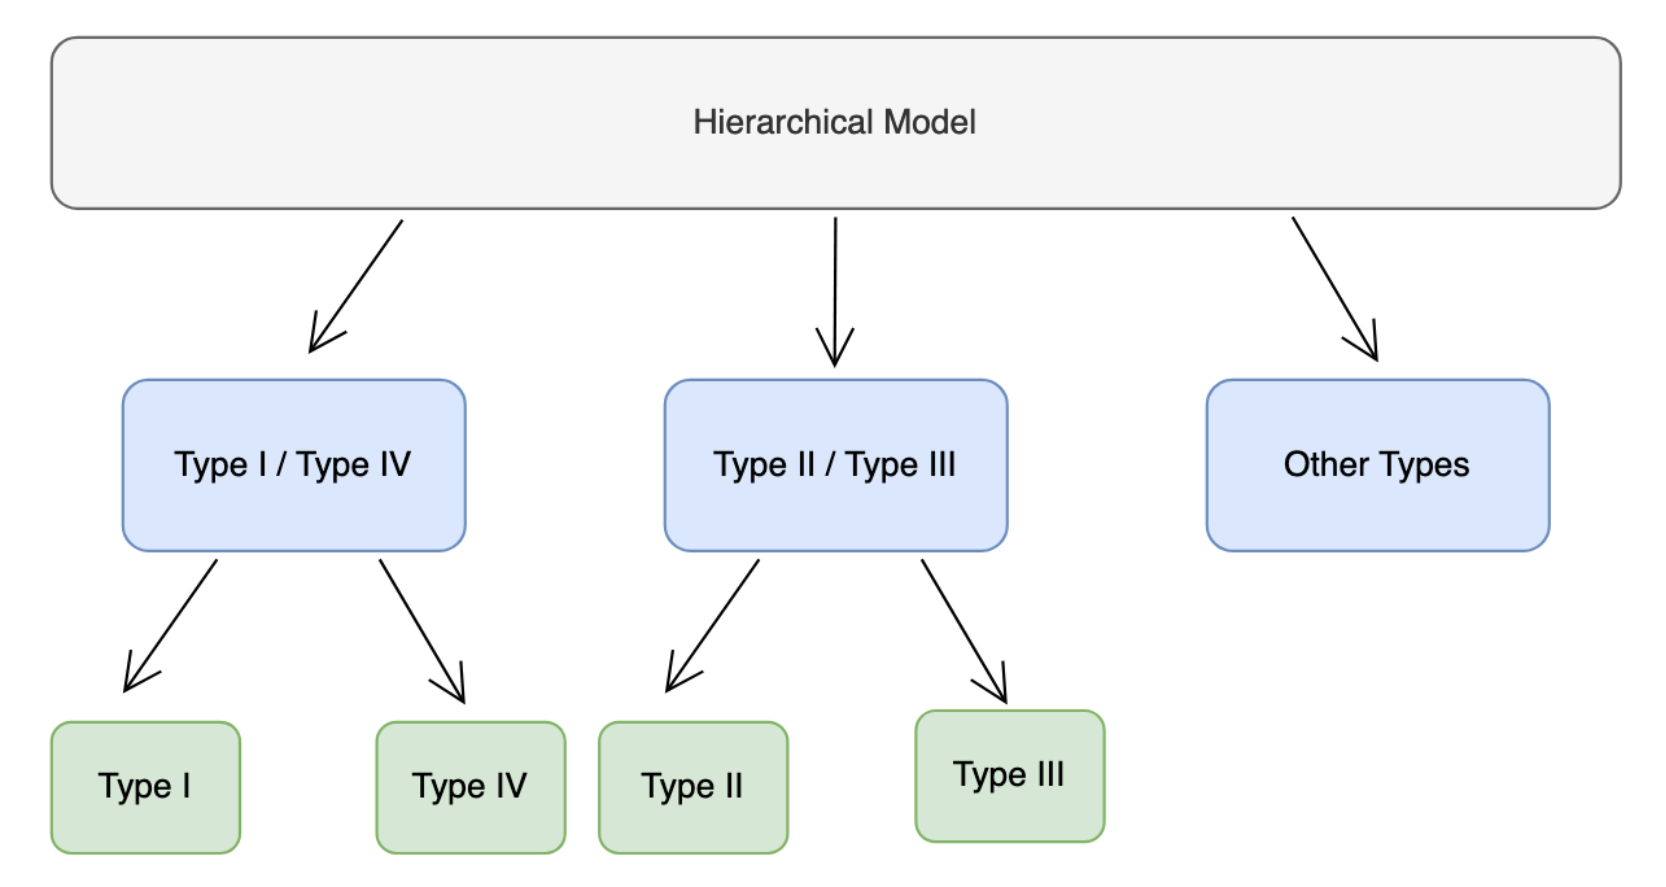
\includegraphics[width=1.1\textwidth]{images/hierarical_model.drawio.png}
	\caption{Architecture behind Hierarchical Models}
	\label{fig:hier_logic}
\end{figure}

\subsection{Additional Approach: BLAST-Based Predictor}
\label{subsection:blast_predictor}
As a baseline method, BLAST (Basic Local Alignment Search Tool) was employed for sequence similarity analysis. To evaluate the predictive power of similarity-based classification, a custom BLAST database was constructed using the training sequences\cite{Altschul1990}.

Each test protein sequence was queried against this database, and the best match was determined based on the lowest e-value, which indicates the statistical significance of the alignment. The predicted label of the matched sequence was then compared to the actual label in the test set to assess the accuracy of this approach.

\subsection{Negative Control: Scrambled Protein Sequence Embeddings}
\label{subsection:negative_control_scrambled_embeddings}

To verify that the machine learning models capture meaningful biological patterns, a negative control was implemented by generating embeddings from scrambled protein sequences. The shuffling of protein sequences was applied while preserving amino acid composition.

For this study, protein sequences were randomly shuffled while preserving their amino acid composition. These scrambled sequences were then processed through the same embedding pipeline using ProtT5 and ProstT5 to generate protein embeddings.